\documentclass[english,floatsintext,man]{apa6}

\usepackage{amssymb,amsmath}
\usepackage{ifxetex,ifluatex}
\usepackage{fixltx2e} % provides \textsubscript
\ifnum 0\ifxetex 1\fi\ifluatex 1\fi=0 % if pdftex
  \usepackage[T1]{fontenc}
  \usepackage[utf8]{inputenc}
\else % if luatex or xelatex
  \ifxetex
    \usepackage{mathspec}
    \usepackage{xltxtra,xunicode}
  \else
    \usepackage{fontspec}
  \fi
  \defaultfontfeatures{Mapping=tex-text,Scale=MatchLowercase}
  \newcommand{\euro}{€}
\fi
% use upquote if available, for straight quotes in verbatim environments
\IfFileExists{upquote.sty}{\usepackage{upquote}}{}
% use microtype if available
\IfFileExists{microtype.sty}{\usepackage{microtype}}{}

% Table formatting
\usepackage{longtable, booktabs}
\usepackage{lscape}
% \usepackage[counterclockwise]{rotating}   % Landscape page setup for large tables
\usepackage{multirow}		% Table styling
\usepackage{tabularx}		% Control Column width
\usepackage[flushleft]{threeparttable}	% Allows for three part tables with a specified notes section
\usepackage{threeparttablex}            % Lets threeparttable work with longtable

% Create new environments so endfloat can handle them
% \newenvironment{ltable}
%   {\begin{landscape}\begin{center}\begin{threeparttable}}
%   {\end{threeparttable}\end{center}\end{landscape}}

\newenvironment{lltable}
  {\begin{landscape}\begin{center}\begin{ThreePartTable}}
  {\end{ThreePartTable}\end{center}\end{landscape}}




% The following enables adjusting longtable caption width to table width
% Solution found at http://golatex.de/longtable-mit-caption-so-breit-wie-die-tabelle-t15767.html
\makeatletter
\newcommand\LastLTentrywidth{1em}
\newlength\longtablewidth
\setlength{\longtablewidth}{1in}
\newcommand\getlongtablewidth{%
 \begingroup
  \ifcsname LT@\roman{LT@tables}\endcsname
  \global\longtablewidth=0pt
  \renewcommand\LT@entry[2]{\global\advance\longtablewidth by ##2\relax\gdef\LastLTentrywidth{##2}}%
  \@nameuse{LT@\roman{LT@tables}}%
  \fi
\endgroup}


  \usepackage{graphicx}
  \makeatletter
  \def\maxwidth{\ifdim\Gin@nat@width>\linewidth\linewidth\else\Gin@nat@width\fi}
  \def\maxheight{\ifdim\Gin@nat@height>\textheight\textheight\else\Gin@nat@height\fi}
  \makeatother
  % Scale images if necessary, so that they will not overflow the page
  % margins by default, and it is still possible to overwrite the defaults
  % using explicit options in \includegraphics[width, height, ...]{}
  \setkeys{Gin}{width=\maxwidth,height=\maxheight,keepaspectratio}
\ifxetex
  \usepackage[setpagesize=false, % page size defined by xetex
              unicode=false, % unicode breaks when used with xetex
              xetex]{hyperref}
\else
  \usepackage[unicode=true]{hyperref}
\fi
\hypersetup{breaklinks=true,
            pdfauthor={},
            pdftitle={Equivalence Testing for Psychological Research: A Tutorial},
            colorlinks=true,
            citecolor=blue,
            urlcolor=blue,
            linkcolor=black,
            pdfborder={0 0 0}}
\urlstyle{same}  % don't use monospace font for urls

\setlength{\parindent}{0pt}
%\setlength{\parskip}{0pt plus 0pt minus 0pt}

\setlength{\emergencystretch}{3em}  % prevent overfull lines

\ifxetex
  \usepackage{polyglossia}
  \setmainlanguage{}
\else
  \usepackage[english]{babel}
\fi

% Manuscript styling
\captionsetup{font=singlespacing,justification=justified}
\usepackage{csquotes}
\usepackage{upgreek}

 % Line numbering
  \usepackage{lineno}
  \linenumbers


\usepackage{tikz} % Variable definition to generate author note

% fix for \tightlist problem in pandoc 1.14
\providecommand{\tightlist}{%
  \setlength{\itemsep}{0pt}\setlength{\parskip}{0pt}}

% Essential manuscript parts
  \title{Equivalence Testing for Psychological Research: A Tutorial}

  \shorttitle{Equivalence Testing Tutorial}


  \author{Daniel Lakens\textsuperscript{1}, Anne M. Scheel\textsuperscript{1}, \& Peder M. Isager\textsuperscript{1}}

  \def\affdep{{"", "", ""}}%
  \def\affcity{{"", "", ""}}%

  \affiliation{
    \vspace{0.5cm}
          \textsuperscript{1} Eindhoven University of Technology  }

 % If no author_note is defined give only author information if available
      \newcounter{author}
                              \authornote{
            Correspondence concerning this article should be addressed to Daniel Lakens, Den Dolech 1, IPO 1.33, 5600 MB, Eindhoven, The Netherlands. E-mail: \href{mailto:D.Lakens@tue.nl}{\nolinkurl{D.Lakens@tue.nl}}
          }
                                                
  \note{\clearpage}

  \abstract{Psychologists must be able to test both for the presence of an effect
and for the absence of an effect. In addition to testing against zero,
researchers can use the Two One-Sided Tests (TOST) procedure to test for
\emph{equivalence} and reject the presence of a smallest effect size of
interest (SESOI). The two one-sided tests procedure can be used to
determine if an observed effect is surprisingly small, given that a true
effect at least as large as the SESOI exists. We explain a range of
approaches to determine the SESOI in psychological science, and provide
detailed examples of how equivalence tests should be performed and
reported. Equivalence tests are an important extension of statistical
tools psychologists currently use, and enable researchers to falsify
predictions about the presence, and declare the absence, of meaningful
effects.}
  \keywords{Equivalence Testing, null-hypothesis significance test, power, TOST,
falsification. \\

    \indent Word count: 5545
  }




  \usepackage{float}
  \usepackage{framed}
  \usepackage{caption}
  \usepackage{setspace}
  \captionsetup[textbox]{name=Box,labelsep=period,labelfont=it}
  \newfloat{textbox}{thp}{lop}
  \floatname{textbox}{Box}

\usepackage{amsthm}
\newtheorem{theorem}{Theorem}
\newtheorem{lemma}{Lemma}
\theoremstyle{definition}
\newtheorem{definition}{Definition}
\newtheorem{corollary}{Corollary}
\newtheorem{proposition}{Proposition}
\theoremstyle{definition}
\newtheorem{example}{Example}
\theoremstyle{definition}
\newtheorem{exercise}{Exercise}
\theoremstyle{remark}
\newtheorem*{remark}{Remark}
\newtheorem*{solution}{Solution}
\begin{document}

\maketitle

\setcounter{secnumdepth}{0}



Psychologists should be able to falsify predictions. A common prediction
in psychological research is that an effect that differs from zero
exists in the population. For example, we might predict that priming
American Asian women with their Asian identity will increase their
performance on a math test compared to women who are primed with their
female identity. To be able to design a study that allows for strong
inferences (Platt, 1964), it is important to specify which test result
would \emph{falsify} this hypothesis.

Equivalence testing can be used to test whether an observed effect is
surprisingly small, assuming a meaningful effect exists in the
population (see for example Goertzen \& Cribbie, 2010; Meyners, 2012;
Quertemont, 2011; Rogers, Howard, \& Vessey, 1993). The test is a simple
variation of widely used null hypothesis significance tests. To
understand the idea behind equivalence tests, it is useful to realize
the null hypothesis we test against can be any numerical value. When we
compare two groups, we often test whether we can reject that the
difference between these groups is zero (see Figure 1A), but we may
sometimes want to reject other values than zero. Imagine a researcher
who is interested in voluntary participation in a national program to
train young infants' motor skills. The researcher wants to test whether
more boys than girls are brought into the program by their parents.
Because the human sex ratio of newborn boys to girls is not exactly 1:1,
we should not expect 50\% of participants to be boys. On average, 103
boys are born for every 100 girls (United States \& Central Intelligence
Agency, 2016), so approximately 50.74\% of applicants should be boys,
and 49.26\% should be girls. If boys and girls were exactly equally
likely to be brought into the program by their parents, we would not
expect a difference of zero, but 50.74\% - 49.26\% = 1.5\% more boys.
Rather than testing against a null hypothesis of 0 difference, the
researcher tests against a null hypothesis of 0.015.

Alternatively, the researcher could decide that even if the true ratio
in the population is not exactly 0.015, the null hypothesis should
consist of a range of values around the difference in proportions of
0.015 that can be considered trivially small. The researcher could for
example test if the difference is smaller than -0.005, or larger than
0.035. This test against two bounds, with \(H_0\) being a range rather
than one value (see Figure 1B), is known as a \emph{minimal effects
test} (Murphy, Myors, \& Wolach, 2014).

\emph{Equivalence tests} can be seen as the opposite of minimal effects
tests: They examine whether the presence of effects that are large
enough to be considered meaningful can be \emph{rejected} (see Figure
1C). Note that when a meaningful effect can be rejected, it does not
imply there is no effect at all. In our example, the researcher can
perform an equivalence test to examine whether the gender difference in
participants is \emph{not} as extreme or more extreme than the
\emph{smallest effect size of interest} (SESOI). After an extensive
discussion with experts, the researcher decides that as long as the
difference in proportions does not deviate from the population gender
ratio by more than 6\%, the gender difference is too small to care
about. Given an expected true difference in the population of 0.015, the
researcher will test if the observed difference falls outside the
boundary values (or \emph{equivalence bounds}) of -0.055 and 0.075. If
differences more extreme than these boundary values can be rejected in
two one-sided tests (TOST), the researcher will conclude statistical
equivalence, the gender difference will be considered trivially small,
and no money will be spent on addressing a gender difference in
participation.

In any one-sided test, for an alpha level of 5\%, we can reject \(H_0\)
when the 90\% confidence interval around the observed estimate is in the
predicted direction, and does not contain the value tested against
(e.g., 0). In the two one-sided tests procedure, the first one-sided
test is used to test against values smaller than the lower equivalence
bound (\(\Delta_{L}\)), and the second one-sided test is used to test
against values larger than the upper equivalence bound (\(\Delta_{U}\)).
Even though the TOST procedure consists of two one-sided tests, it is
not necessary to control for multiple comparisons because both tests
need to be statistically significant to conclude equivalence.
Consequently, when reporting an equivalence test, it suffices to report
the one-sided test with the smaller test parameter (e.g. \(t\) or \(r\))
and thus the larger \(p\)-value. Statistical equivalence can be
concluded when the largest of the two \(p\)-values is smaller than
alpha. If results are neither statistically different from zero nor
statistically equivalent, there is insufficient data to draw
conclusions. Further studies are needed, which can be analyzed using a
(small-scale) meta-analysis. The additional data will narrow the
confidence interval around the observed effect, allowing us to reject
the null, reject the SESOI, or both. Analogous to the large sample sizes
needed to detect small effects, as the SESOI becomes smaller, the
equivalence bounds become narrower, and the sample size needed to obtain
a sufficiently narrow confidence interval increases.

Note that in this paper we will control the Type 1 error rate at 5\% for
all examples, mirroring the studies we reanalyze (but we recommend to
justify the Type 1 error rate in original research based on substantive
arguments, Lakens et al., 2017). It may be easiest to think of an
equivalence test as checking whether the entire 90\% confidence interval
falls entirely between the upper and lower equivalence bounds, but for
any given study an equivalence test could also be conceptualized as
determining whether effect sizes or test statistics are closer to zero
than some critical value, or even whether the \emph{p}-value for a
null-hypothesis significance test is larger than some \emph{p}-value
bound.

\begin{figure}
\centering
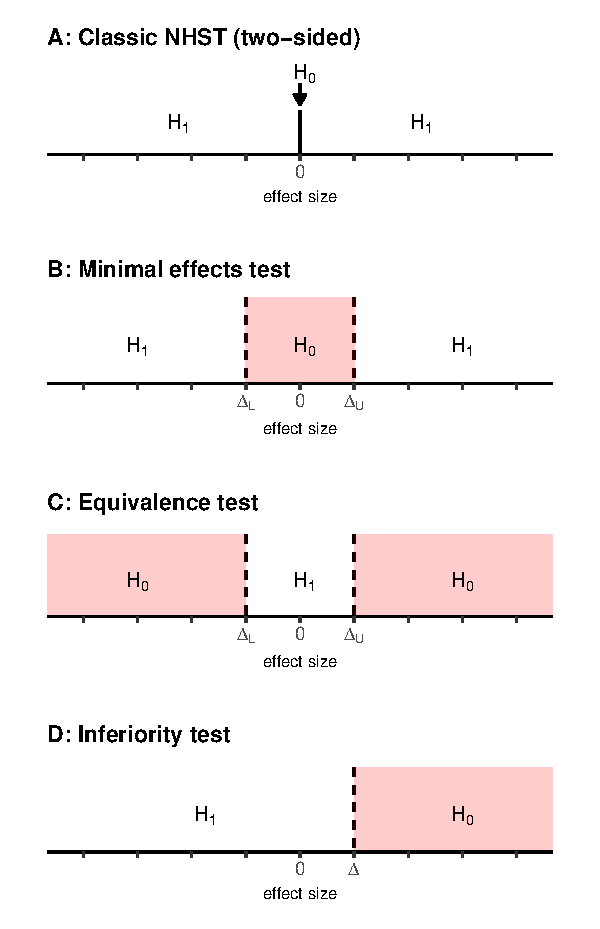
\includegraphics{Figure_1.pdf}
\caption{\label{fig:unnamed-chunk-2}Illustration of null hypotheses
(\(H_0\)) and alternative hypotheses (\(H_1\)) for different types of
significance tests. \textbf{A)} Null-Hypothesis Significance Test: Tests
if the hypothesis (\(H_0\)) that an effect is equal to 0 can be
rejected. \textbf{B)} Minimal effects test: Tests if the hypothesis
(\(H_0\)) that an effect is larger than \(\Delta_{L}\) \emph{and}
smaller than \(\Delta_{U}\) can be rejected. \textbf{C)} Equivalence
test: Tests if the hypothesis (\(H_0\)) that an effect is smaller than
\(\Delta_{L}\) \emph{or} larger than \(\Delta_{U}\) can be rejected.
\textbf{D)} Inferiority test: Tests if the hypothesis (\(H_0\)) that an
effect is larger than \(\Delta\) can be rejected.}
\end{figure}

In this article we provide five reproducible examples of equivalence
tests which illustrate the procedure in free, easy-to-use software (R,
jamovi, and a spreadsheet). But first, we discuss different approaches
to determining the smallest effect size of interest for psychological
research, which determines the statistical question an equivalence test
answers.

\section{Justifying the Smallest Effect Size of
Interest}\label{justifying-the-smallest-effect-size-of-interest}

The Two One-Sided Test procedure is performed against equivalence bounds
that are considered the smallest effect size of interest. The smallest
effect size of interest (SESOI) can sometimes be determined objectively
(for example based on just noticeable differences, as we will explain
below). In lieu of objective justifications, the SESOI should ideally be
based on a cost-benefit analysis. Since both costs and benefits are
necessarily subjective, the SESOI will vary across researchers, fields,
and time. The goal of setting a SESOI is to clearly justify why
designing a study that has a high probability of rejecting effects more
extreme than the specified equivalence bounds contributes to our
knowledge base. The SESOI is thus independent of the outcome of the
study, and should be determined before looking at the data. A SESOI
should be chosen such that inferences based on it answer a meaningful
question. Although we use bounds that are symmetric around 0 for all
equivalence tests in this manuscript (e.g., \(\Delta_{L} = -0.3\),
\(\Delta_{U} = 0.3\)), it is also possible to use asymmetric bounds
(e.g., \(\Delta_{L} = -0.2\), \(\Delta_{U} = 0.3\)).

\subsection{Objective Justification of a Smallest Effect Size of
Interest}\label{objective-justification-of-a-smallest-effect-size-of-interest}

An objectively determined smallest effect size of interest (SESOI)
should be based on quantifiable theoretical predictions, such as
computational models. Sometimes, the only theoretical prediction is that
an effect should be noticeable. In such circumstances, the SESOI can be
set based on just noticeable differences. For example, Burriss and
colleagues (2015) examined whether women displayed an increase in
redness in the face during the fertile phase of their ovulatory cycle.
The hypothesis was that a slightly redder skin signals greater
attractiveness and physical health, and sending this signal to men
yields an evolutionary advantage. This hypothesis presupposes that men
can detect the increase in redness with the naked eye. Burriss and
colleagues collected data from 22 women and showed that there was indeed
an increase in redness of the facial skin during their fertile period.
However, this increase was not large enough for men to detect with the
naked eye, thus falsifying their hypothesis. Because the just noticeable
difference in redness of the skin can be measured, it is possible to
establish an objective SESOI.

Another example of an objectively determined SESOI can be found in
Button et al. (2015), where the minimal clinically important difference
on the Beck Depression Inventory -- II was determined by asking 1039
patients when they subjectively felt less depressed (i.e., when they
personally noticed an improvement) and relating this to the
corresponding difference score on the depression inventory. Similarly,
Norman, Sloan, and Wyrwich (2003) proposed there is a surprisingly
consistent minimally important difference of half a standard deviation,
or \(d = 0.5\), in health outcomes.

\subsection{Subjective Justification of a Smallest Effect Size of
Interest}\label{subjective-justification-of-a-smallest-effect-size-of-interest}

We distinguish between three categories of subjective justifications to
determine the smallest effect size of interest. First, researchers can
use benchmarks. For example, one might set the smallest effect size of
interest to a standardized effect size of \(d = 0.5\), which would allow
rejecting effects more extreme than a \enquote{medium} effect size
(Cohen, 1988). Similarly, effect sizes smaller than a Cohen's \(d\) of
0.1 are sometimes considered trivially small (Maxwell, Lau, \& Howard,
2015). Relying on a benchmark is the weakest possible justification of a
smallest effect size of interest, and should be avoided. Based on a
review of 112 meta-analyses, Weber and Popova (2012) conclude that
setting a smallest effect size of interest (SESOI) to a medium effect
size (\(r = 0.3\), or \(d = 0.5\)) corresponds to rejecting only the
upper 25\% of effect sizes reported in communications research, and
Hemphill (2003) suggests that a smallest effect size of interest of
\(d = 0.5\) would imply rejecting effects as large as the upper 33\% of
effect sizes reported in the psychological literature.

Second, the SESOI can be based on related published studies in the
literature. Ideally, researchers who publish novel research would always
specify their smallest effect size of interest, but this is not yet
common practice. It is thus up to researchers who build on earlier work
to decide which effect size is too small to be meaningful when examining
the same hypothesis. Simonsohn (2015) recently proposed to set the SESOI
to the effect size that an earlier study would have had 33\% power to
detect. With this so-called \enquote{small telescopes} approach, the
equivalence bounds are thus primarily based on the sample size in the
original study. For example, consider a study in which 100 participants
answered a question, and the results were analyzed with a one-sample
t-test. For a two-sided test with an alpha of 0.05, this test had 33\%
power to detect an effect of \(d = 0.15\). Another example of how
previous research can be used to determine the SESOI can be found in
Kordsmeyer and Penke (2017), who defined the SESOI based on the mean of
effect sizes reported in the literature. Thus, they examined whether
their replication study could reject effects as large or larger than had
on average been reported in the literature. Given random variation and
bias in the literature, a more conservative approach could be to use the
lower end of a confidence interval around the meta-analytic effect size
estimate (cf. Perugini, Gallucci, \& Costantini, 2014).

Another justifiable option when choosing the SESOI based on earlier work
is to use the smallest observed effect size that could have been
statistically significant in a previous study. In other words, we decide
that effects that could not have yielded a \(p < \alpha\) in an original
study will not be considered meaningful in the replication study either,
even if they were found to be statistically significant. The assumption
here is that authors were interested in observing a significant effect,
and thus were not interested in observed effect sizes that could not
have yielded a significant effect. It might be likely that the original
authors did not consider which effect sizes they could detect at all, or
that they were interested in smaller effects, but gambled on observing
an especially large effect in the sample purely due to random variation.
Even then, observed effect sizes that could not have been significant in
an earlier study might be a justifiable starting point when building on
earlier research that did not specify a smallest effect size of
interest. Based only on the alpha level and the sample size, we can
calculate the critical test value (e.g., \emph{t}, \emph{F}, \emph{Z}).
This critical test value can be transformed to a standardized effect
size (e.g.,
\(d = t \sqrt { \frac { 1} { n _ { 1} } + \frac { 1} { n _ { 2} } }\)),
which can thus be interpreted as the \emph{critical effect
size}.\footnote{This will typically, although not always, correspond to
  the effect size the study had 50\% power to detect (see Lenth, 2007).
  This procedure will result in equivalence bounds that are wider than
  the ones obtained using the small telescopes approach, which gives the
  effect size a study had 33\% power to detect.} All observed effect
sizes smaller than the critical effect size would not have been
statistically significant in the original study, given the alpha and
sample size of that study. By setting the SESOI to the critical effect
size, an equivalence test can reject all observed effect sizes that
could have been detected in an earlier study.

Third, the SESOI can be determined based on a \emph{resource} question.
Not all psychological theories make quantifiable predictions (possibly
related to the strong reliance on null-hypothesis significance testing
in some fields, see Meehl, 1978). Researchers often have more precise
ideas of the amount of data that they can afford to collect, or that
other researchers in their field commonly collect. The amount of data
that is collected limits the inferences you can make. Given the alpha
level and the planned sample size, researchers can calculate the
smallest effect size that they have sufficient power to
detect.\footnote{This approach is conceptually very similar to the
  \emph{power approach}, where the effect size you had 95\% power to
  detect is calculated, and the presence of effects more extreme than
  this value is rejected after observing a \(p\)-value \emph{larger
  than} 0.05 in a traditional null-hypothesis significance test.
  However, Meyners (2012) explains that this approach is not recommended
  (even though it is common) because it ignores the possibility that
  effects are significant \emph{and} equivalent, and error rates are not
  controlled accurately.}

An equivalence test based on this approach does not answer any
theoretical question (after all, the equivalence bounds are not based on
any theoretical predictions). When theories only allow for directional
predictions, but do not predict effects of a specific size, the sample
size justification can be used to determine which effects can be studied
reliably, and thus which effects would be interesting to reject. For
example, imagine a research line where almost all studies examined a
hypothesis by performing a one-sample \(t\)-test on sample sizes smaller
than 100. A one-sample \(t\)-test using an alpha of 5\% (two-sided) with
100 observations has 90\% power to detect an effect of \(d = 0.33\).
Concluding equivalence in a test using equivalence bounds of
\(\Delta_{L} = -0.33\) and \(\Delta_{U} = 0.33\) would suggest that
effects as large or larger than those which published studies were
sensitive enough to detect can be rejected. Such a study does not test a
theoretical prediction, but it contributes to the literature by
suggesting much larger sample sizes than 100 observations are needed.

When there is no previous literature on a topic, researchers can justify
their sample size based on reasonable resource limitations, which are
specific to scientific disciplines and research questions (and can be
expected to change over time). Where 22 patients with a rare
neurological disorder might be the largest sample a single researcher
can collect, a study on mTurk might easily collect hundreds or thousands
of observations. Thus, whether or not the resource question that is
answered by an equivalence test is interesting must be evaluated by
peers, preferably when the study design is submitted to an ethical
review board or as a Registered Report.

Additional subjective justifications for a smallest effect size of
interest are possible. For example, the Food and Drug Administration has
set equivalence bounds for bioequivalence studies, taking the decision
out of the hands of individual researchers (Senn, 2007). We have
provided several approaches to help researchers justify equivalence
bounds, but want to repeat the warning by Rogers et al. (1993), p.~564:
\enquote{The thoughtless application of \enquote{cookbook} prescriptions
is ill-advised, regardless of whether the goal is to establish a
difference or to establish equivalency between treatments}. By
transparently reporting and adequately justifying the smallest effect
size of interest, researchers can communicate the information their
study contributes to the literature, and provide a starting point for a
discussion about what a reasonable SESOI may be.

\subsection{Raw Versus Standardized Equivalence
Bounds}\label{raw-versus-standardized-equivalence-bounds}

The SESOI, and thus the equivalence bounds, can be set in terms of
standardized effect sizes (e.g.~a Cohen's \(d\) of 0.5) or as a raw mean
difference (e.g.~0.5 points on a 7-point scale). The key difference is
that equivalence bounds set in raw differences are independent of the
standard deviation, while equivalence bounds set as standardized effects
are dependent on the standard deviation (since they are calculated as
\(\frac {X _ { 1} - X _ { 2} } {S D}\)). The observed standard deviation
randomly varies across samples. In practice, this means that when using
standardized differences as bounds (e.g., \(d = 0.35\)), the equivalence
test depends on the standard deviation in the sample. The equivalence
bound for a raw mean difference of 0.5 equals a standardized equivalence
bound of \(d = 0.5\) when the standard deviation is 1, but a
standardized equivalence bound of \(d = 1\) when the standard deviation
is 0.5.

Both raw equivalence bounds and standardized equivalence bounds have
specific benefits and limitations (for a discussion, see Baguley, 2009).
When raw mean differences are meaningful and of theoretical interest, it
makes sense to set equivalence bounds based on raw effect sizes. When
the raw mean difference is of less theoretical importance, or different
measures are used across research lines, it is often easier to set
equivalence bounds based on standardized differences. Researchers should
realize that equivalence bounds based on raw differences or standardized
differences ask slightly different questions, and justify their choice
for either option. When setting equivalence bounds based on earlier
research, such as in replication studies, equivalence bounds based on
raw or standardized differences would ideally give the same result, and
large differences in standard deviations between studies are as
important to interpret as large differences in means.

In the remainder of this article we will provide five detailed examples
of equivalence tests performed on published studies. These concrete and
easy to follow examples will illustrate all approaches to setting
equivalence bounds discussed above, and demonstrate how to perform and
report equivalence tests.

\begin{figure}
\centering
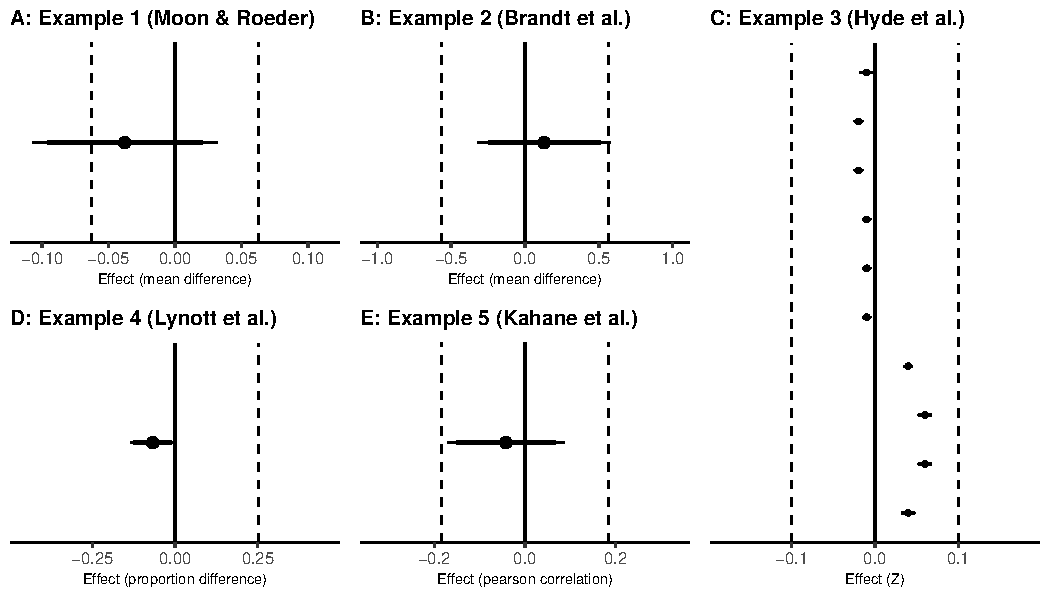
\includegraphics{Figure_2.pdf}
\caption{\label{fig:unnamed-chunk-6}Example effects plotted with 90\% two
one-sided tests confidence intervals (thick lines) and 95\%
null-hypothesis significance test confidence intervals (thin lines), the
null hypothesis (solid vertical line) and the equivalence bounds (dashed
vertical lines) displayed. \textbf{A)} Example 1 - Mean Difference.
\textbf{B)} Example 2 - Mean Difference. \textbf{C)} Example 3 -
Meta-analytic Effect Size. \textbf{D)} Example 4 - Proportion
Difference. \textbf{E)} Example 5 - Pearson Correlation.}
\end{figure}

\subsection{Example 1: Not Statistically Equivalent and Not
Statistically
Different}\label{example-1-not-statistically-equivalent-and-not-statistically-different}

Moon and Roeder (2014), replicating Shih, Pittinsky, and Ambady (1999),
conducted a study to investigate whether Asian-American women would
perform better on a maths test when primed with their Asian identity. In
contrast to the original study, they found a negative difference between
the Asian primed group (\(n = 53\), \(M = 0.46\), \(SD = 0.17\)) and the
control (\(n = 48\), \(M = 0.50\), \(SD = 0.18\)) which was not
significant, \(d = -0.21\), \(t(97.77) = -1.08\), \(p = .284\),
two-sided\footnote{Fractional degrees of freedom in \emph{t}-tests are a
  result of using Welch's \emph{t}-test instead of Student's
  \emph{t}-test, which is the recommended default when sample sizes are
  unequal between groups (Delacre, Lakens, \& Leys, 2017). When using
  the TOSTER package in R, this is achieved by setting
  \enquote{var.equal = FALSE}.}. The non-significant null-hypothesis
test does not allow us to distinguish between the absence of a
meaningful effect and data that are not sensitive enough to tell us
whether a meaningful effect is present or absent.

In order to distinguish between these possibilities, we can define what
a \enquote{meaningful effect} would be and use it as the bounds for an
equivalence test (remember that these bounds should normally be
specified before looking at the data). If grades for this test were set
at every 6.25\% increase in correct answers (F = 0\% to 6.25\%, \ldots{}
A+ = 93.75\% to 100\%) we could decide that we are only interested in
test score differences that correspond to an increase or decrease of at
least 1 grade point. Thus, our SESOI becomes a difference in raw scores
of 6.25\%, or 0.0625. We can then perform an equivalence test for a
two-sample Welch's \emph{t}-test, with equivalence bounds of \(\pm\) the
SESOI of 0.0625. The two one-sided-tests procedure consists of two
one-sided tests, and we calculate \emph{t}-values and \emph{p}-values
both for the test against \(\Delta_{L}\), \(t(97.77) = 0.71\),
\(p = .241\), and \(\Delta_{U}\), \(t(97.77) = -2.86\), \(p = .003\).
While the \emph{t}-test against \(\Delta_{U}\) indicates that we can
reject differences at least as extreme as 0.0625, the test against
\(\Delta_{L}\) shows we can \emph{not} reject effects as extreme or more
extreme than -0.0625. The equivalence test is therefore non-significant,
which means we cannot reject a true effect as large or larger than
6.25\% (Figure 2A), \(t(97.77) = 0.71\), \(p = .241\) (note we typically
only report the one-sided test yielding the higher \emph{p}-value in the
result section).\footnote{Because this is a replication of a study, it
  would have been reasonable to assume that we only want to reject
  effects in the same direction as the effect in the original study.
  After all, much smaller effects may indicate non-replication, but so
  do large effects in the opposite direction. In that case, we would
  perform an inferiority test (see figure 1D) against \(\Delta_{U}\). As
  can be seen in Figure 2A, the 90\% CI does not overlap with
  \(\Delta_{U}\), so we can reject effects as large or larger than
  \(0.0625\). However, this must be decided before running the tests to
  prevent loss of error control.}

\subsection{Example 2: Statistically Equivalent and Not Statistically
Different}\label{example-2-statistically-equivalent-and-not-statistically-different}

Banerjee, Chatterjee, and Sinha (2012) reported that 40 participants who
had been asked to describe an unethical deed from their past judged the
room to be darker than participants who had been asked to describe an
ethical deed (\(t(38)= 2.03\), \(p= .049\), \(d= 0.65\)). A close
replication by Brandt, IJzerman, and Blanken (2014) with 100
participants found no significant effect (\(M_{unethical}= 4.79\),
\({SD}_{unethical}= 1.09\), \(M_{ethical}=4.66\),
\({SD}_{ethical}=1.19\), \(t(97.78)=0.57\), \(p=.573\), \(d=0.11\)). We
can choose (before looking at the data) to use the small telescopes
approach, calculate the effect size the original study had 33\% power to
detect (\(d = 0.49\)), and use this effect size as the equivalence
bounds. The two one-sided tests procedure for Welch's \emph{t}-test for
independent samples and equivalence bounds of \({\Delta}_L=-0.49\) and
\({\Delta}_U=0.49\) reveals that the effect observed in the replication
study is statistically equivalent, because the larger of the two p
values was less than .05, \(t(97.78)=-1.90\), \(p=.030\) (Figure 2B).
Following a Neyman-Pearson approach, this means we can reject the
hypothesis that the true effect is smaller than \(d = -0.49\) or larger
than \(d = 0.49\), and we can act as if the effect size falls within the
equivalence bounds, with the understanding that based on our chosen
alpha level, we will not be wrong more than 5\% of the time.

\subsection{Example 3: Statistically Equivalent and Statistically
Different}\label{example-3-statistically-equivalent-and-statistically-different}

Hyde, Lindberg, Linn, Ellis, and Williams (2008) reported that effect
sizes for gender differences in mathematics tests across the 7 million
students in the US represent trivial differences, which the authors
specify as absolute effect sizes smaller than \(d = 0.10\). For example,
in grade 3 the difference is \(d = 0.04\), with a standard error of
0.002. When we perform equivalence tests on the meta-analytic effect
sizes of IQ difference for grades 2 to 11 (using an alpha level of .005
to correct for multiple comparisons) and using equivalence bounds of
\(\Delta_{L} = -0.1\) and \(\Delta_{U} = 0.1\), we see that all effect
size estimates are measured with such high precision that they are
statistically equivalent, and can be considered trivially small
according to the authors' definition (Figure 2C). In the case of grade
3, \(z = 70.00\), \(p < .001\). However, note that all of the effects
are also statistically different from zero, as one might expect when
there is no random assignment to conditions and samples sizes are very
large (e.g., for grade 3, \(z = 20.00\), \(p < .001\)). We see how
equivalence tests allow researchers to distinguish between
\emph{statistical} significance and \emph{practical} significance, which
demonstrates how equivalence tests improve hypothesis testing procedures
in psychological research.

\subsection{Example 4: Statistically Inferior and Not Statistically
Different}\label{example-4-statistically-inferior-and-not-statistically-different}

Lynott et al. (2014) conducted a study to investigate the effect of
being exposed to physically warm or cold stimuli on subsequent judgments
related to interpersonal warmth and prosocial behavior (replicating L.
E. Williams \& Bargh, 2008). They observed that 50.74\% of participants
who received a cold pack (\(n_{cold}=404\)) opted to receive a reward
for themselves, while 57.46\% of participants who received a warm pack
(\(n_{hot}=409\)) did the same. In a \emph{z}-test for the difference
between the proportions, this effect is not statistically significant
(\(\mathit{Diff}=-6.71\)\%, \(z=-1.93\), \(p=.054\)). Had the authors
planned to perform a null-hypothesis significance test \emph{and} an
equivalence test, the latter would allow one to distinguish between an
inconclusive outcome, or a statistically equivalent result.

Since this is a replication, we could decide in advance that we are
interested in whether the observed effect size is smaller than the
smallest effect size that the original study could have detected. This
means that we use the critical \emph{z} value (\textasciitilde{}1.96 in
a two-tailed test with an alpha of 0.05) as equivalence bounds
(\(\Delta = \pm 1.96\)). To calculate which difference corresponds to a
critical \emph{z} value in the original study, we multiply the critical
\emph{z} value with the standard error (\(1.96\) * \(0.13\)), and find
that the original study could have observed a significant effect for
differences of \(0.25\) or more. Since the original study had a clear
directional hypothesis, in this replication study we are only interested
in whether receiving a warm pack \emph{increases} the proportion of
people who choose a gift for a friend. This means we can test for
inferiority (see Figure 1D) and conclude the absence of a meaningful
effect if the observed effect size is reliably \emph{lower} than the
SESOI. We find that we can reject effects larger than
\(\Delta_{U} = 0.25\), \(z = -9.12\), \(p < .001\) (see Figure 2D).
Thus, we can conclude that the statistically non-significant effect is
also statistically smaller than our SESOI.

\subsection{Example 5: Statistically Equivalent and not Statistically
Different}\label{example-5-statistically-equivalent-and-not-statistically-different}

Kahane and colleagues (2015) investigated how responses to moral
dilemmas in which participants have to decide whether or not they would
sacrifice one person's life to save several other lives relate to other
indicators of moral orientation. Traditionally, greater endorsement for
sacrificing one life to save several others has been interpreted as a
more \enquote{utilitarian} moral orientation (i.e.~a stronger concern
for the greater good). Kahane et al. contest this interpretation in a
number of studies. In Study 4, they compare the traditionally used
dilemmas with a set of new dilemmas in which the sacrifice for the
greater good is not another person's life, but something the participant
would have a partial interest in (e.g.~buying a new mobile phone
vs.~donating the money to save lives in a distant country). The authors
find no significant correlation between the two sets of dilemmas,
\(r(229) = -0.04\), \(p = .525\), \(N = 231\)\footnote{Study 4 in Kahane
  et al. (2015) had a final sample size of \(N = 232\), but due to
  missing data in 1 case, the correlation reported here is based on a
  sample of \(N = 231\).}. The authors conclude that \enquote{a robust
association between \enquote{utilitarian} judgment and genuine concern
for the greater good seems extremely unlikely} (p.~206), given the
statistical power their study had to detect meaningful effect sizes.

This interpretation can be formalized by performing an equivalence test
for correlations, where equivalence bounds are set to an effect size the
study had reasonable power to detect (as decided before looking at the
data). With 231 participants, the study had 80\% power to detect effects
of \(r = 0.18\). Performing the two one-sided tests procedure given
bounds of \(\Delta_{L} = -0.18\) and \(\Delta_{U} = 0.18\), the data is
statistically equivalent, \(r(229) = -0.04\), \(p = .015\). This means
that values smaller than \(r = -0.18\) and larger than \(r = 0.18\) can
be rejected at an alpha level of 5\%. If other researchers are
interested in examining the presence of a smaller effect size, they can
design studies with a larger sample size.

\begin{textbox}
\caption{Calculating an equivalence test in R.}
\begin{framed}
{\sffamily \small \setstretch{1}
Equivalence tests can be performed  based on summary statistics (e.g., means, standard deviations, and sample sizes) with the ``TOSTER'' package in the open-source programming language R. Using TOSTER in R requires no more programming experience than reproducing three lines of code.
\vspace{2mm}

The code below reproduces the result of Example 2 in R, which can be typed into R or RStudio. The parameters of the test are defined inside the parentheses. Simply copy the example to the console, replace the values with the corresponding values of your own study, and run the code. Results and a plot will automatically be printed. A help file provides more detailed information.

\begin{verbatim}
install.packages("TOSTER")

library(TOSTER)

TOSTtwo(m1 = 4.7857, m2 = 4.6569, sd1 = 1.0897, sd2 = 1.1895, n1 = 49,
n2 = 51, low_eqbound_d = -0.6401696, high_eqbound_d = 0.6401696, alpha = 0.05,
var.equal = FALSE)
\end{verbatim}
}
\end{framed}
\end{textbox}

\section{Discussion}\label{discussion}

Equivalence testing is a simple statistical technique to reject the
presence of a smallest effect size of interest. As long as we can
calculate a confidence interval around a parameter estimate, we can
compare it to the SESOI. The result of an equivalence test can be
obtained by mere visual inspection of the CI (Seaman \& Serlin, 1998;
Tryon, 2001), or by performing two one-sided tests (known as the TOST
procedure).

As with any statistical test, the usefulness of the result of an
equivalence test depends on the question we ask. The question manifests
itself in the bounds we set: Is our data surprisingly close to zero,
assuming a true effect exists that is as large as our smallest effect
size of interest? If we test against very wide bounds, observing
statistical equivalence can hardly be considered surprising, given that
most effects in psychology are small to medium (Hemphill, 2003).
Examining papers citing Lakens (2017a), we found that some researchers
state, but do not justify, the SESOI used in the equivalence test (e.g.,
Brown, Rodriguez, Gretak, \& Berry, 2017; Schumann, Klein, Douglas, \&
Hewstone, 2017). An equivalence test using a SESOI of \(d = 0.5\) might
very well answer a question the researchers are interested in (for one
possible justification based on minimally important differences, see
Norman et al., 2003), but researchers should always explain why they
chose a SESOI. It makes little sense to report a statistical test
without explaining why one would want to answer this question to begin
with.

Equivalence bounds should be specified before results are known, ideally
as part of a preregistration (cf. Piaggio et al., 2006). In the most
extreme case, a researcher can always first look at the data, and then
choose equivalence bounds wide enough for the test to yield a
\enquote{statistically equivalent} result (for a discussion, see Weber
\& Popova, 2012). However, fixed error rates are no longer valid when
bounds are determined based on the observed data. The value of reporting
an equivalence test is determined by the strength of the justification
of the equivalence bounds. If bounds are chosen based on the observed
data, an equivalence test becomes meaningless. We have proposed several
ways to justify equivalence bounds, but in the end these discussions
must happen among peers, and the best place for these discussions is
during peer-review of proposals for Registered Reports.

As with null-hypothesis significance tests, equivalence tests
interpreted from a Neyman-Pearson perspective on statistical inferences
are used to guide the actions of researchers while controlling error
rates. Research lines sometimes require dichotomous choices. For
example, a researcher might want to decide to discontinue a research
line when an effect is too small to be considered meaningful.
Equivalence tests based on carefully chosen equivalence bounds and error
rates can be used as a rule to govern our behavior (Neyman \& Pearson,
1933). An equivalence test and a null-hypothesis significance test
examine two different hypotheses, and can therefore be used in concert
(Weber \& Popova, 2012). We recommend that researchers by default
perform both a null hypothesis significance test \emph{and} an
equivalence test on their data, as long as they can justify a smallest
effect size of interest, in order to improve the falsifiability of
predictions in psychological science.

The biggest challenge for researchers will be to specify the smallest
effect size of interest. Psychological theories are usually too vague to
derive precise predictions, and if there are no theoretical reference
points, natural constraints, or prior studies a researcher can use to
define the SESOI for a hypothesis test, any choice will be somewhat
arbitrary. In some research lines, researchers might use equivalence
tests to simply reject consecutively smaller effect sizes by performing
studies with increasingly large sample sizes while controlling error
rates, until no one is willing to invest the time and resources needed
to examine the presence of even smaller effects. Nevertheless, it is
important to realize that not specifying a SESOI for our research
questions at all will severely hinder theoretical progress (Morey \&
Lakens, 2016). Incorporating equivalence tests in our statistical
toolbox will in time contribute to better --- and more falsifiable ---
theories.

\newpage

\subsection{Disclosures}\label{disclosures}

\subsubsection{Data, materials, and online
resources}\label{data-materials-and-online-resources}

The code to reproduce these analyses is available at
\url{https://osf.io/qamc6/}. The OSF project contains all necessary
files to reproduce examples 1--5 in R, jamovi (jamovi project, 2017),
and in a spreadsheet; as well as a preprint of this manuscript. The
manuscript, including the figures and statistical analyses, was created
using RStudio (1.1.383, RStudio Team, 2016) and R (3.4.2, R Core Team,
2017) and the R-packages \emph{bookdown} (0.5, Xie, 2016),
\emph{ggplot2} (2.2.1, Wickham, 2009), \emph{gridExtra} (2.3, Auguie,
2017), \emph{knitr} (1.17, Xie, 2015), \emph{lattice} (0.20.35, Sarkar,
2008), \emph{papaja} (0.1.0.9492, Aust \& Barth, 2017), \emph{purrr}
(0.2.4, Henry \& Wickham, 2017), \emph{pwr} (1.2.1, Champely, 2017),
\emph{rmarkdown} (1.7, Allaire et al., 2017), and \emph{TOSTER} (0.3,
Lakens, 2017b). \newline

\subsubsection{Conflicts of Interest}\label{conflicts-of-interest}

The authors declare that they have no conflicts of interest with respect
to the authorship or the publication of this article. \newline

\subsubsection{Author Contributions}\label{author-contributions}

DL: Article conceptualization, programming TOSTER package and
spreadsheet, main contributor to the introduction section and discussion
section. AMS and PMI: Main contributors to examples and figures. All
authors contributed to manuscript conceptualization, editing, review for
submission, and additional software development. AMS and PMI contributed
equally to the manuscript, and order was determined by executing the
following commands in R: \newline
 \texttt{set.seed(7998976/5271)} \newline
 \texttt{x\ \textless{}-\ sample(c("Anne",\ "Peder"),\ 1)} \newline
 \texttt{print(paste("The\ winner\ is",\ x,\ "!"))} \newline

\subsubsection{Acknowledgments}\label{acknowledgments}

This work was funded by VIDI grant 452-17-013. We would like to thank
Courtney Soderberg for creating the first version of the TOST function
to test two independent proportions, Dermot Lynott and Katie Corker for
their helpful responses to our inquiries about Lynott et al. (2014), Jim
Everett and Brian Earp for their helpful responses and for providing the
raw data for study 4 in Kahane et al. (2015), and Neil McLatchie and Jan
Vanhove for valuable comments on an earlier version of this manuscript.
\newline

\subsubsection{Prior versions}\label{prior-versions}

A preprint version of this manuscript prior to peer-review can be found
on PsyArxiv: \url{https://psyarxiv.com/v3zkt/} (version 1). We have
updated our recommendations on how to justify the SESOI based on
available resources. The updated preprint version (version 2) is
identical in content to the published manuscript.

\newpage

\section{References}\label{references}

\setlength{\parindent}{-0.5in} \setlength{\leftskip}{0.5in}

\hypertarget{refs}{}
\hypertarget{ref-R-rmarkdown}{}
Allaire, J., Xie, Y., McPherson, J., Luraschi, J., Ushey, K., Atkins,
A., \ldots{} Chang, W. (2017). \emph{rmarkdown: Dynamic documents for
R}. Retrieved from \url{https://CRAN.R-project.org/package=rmarkdown}

\hypertarget{ref-R-gridExtra}{}
Auguie, B. (2017). \emph{gridExtra: Miscellaneous functions for ``grid''
graphics}. Retrieved from
\url{https://CRAN.R-project.org/package=gridExtra}

\hypertarget{ref-R-papaja}{}
Aust, F., \& Barth, M. (2017). \emph{papaja: Create APA manuscripts with
R Markdown}. Retrieved from \url{https://github.com/crsh/papaja}

\hypertarget{ref-Baguley2009}{}
Baguley, T. (2009). Standardized or simple effect size: What should be
reported? \emph{British Journal of Psychology}, \emph{100}(3), 603--617.
doi:\href{https://doi.org/10.1348/000712608X377117}{10.1348/000712608X377117}

\hypertarget{ref-Banerjee2012}{}
Banerjee, P., Chatterjee, P., \& Sinha, J. (2012). Is It Light or Dark?
Recalling Moral Behavior Changes Perception of Brightness.
\emph{Psychological Science}, \emph{23}(4), 407--409.
doi:\href{https://doi.org/10.1177/0956797611432497}{10.1177/0956797611432497}

\hypertarget{ref-Brandt2014}{}
Brandt, M. J., IJzerman, H., \& Blanken, I. (2014). Does Recalling Moral
Behavior Change the Perception of Brightness?: A Replication and
Meta-Analysis of Banerjee, Chatterjee, and Sinha (2012). \emph{Social
Psychology}, \emph{45}(3), 246--252.
doi:\href{https://doi.org/10.1027/1864-9335/a000191}{10.1027/1864-9335/a000191}

\hypertarget{ref-Brown2017}{}
Brown, M., Rodriguez, D. N., Gretak, A. P., \& Berry, M. A. (2017).
Preliminary Evidence for How the Behavioral Immune System Predicts Juror
Decision-Making. \emph{Evolutionary Psychological Science}, \emph{3}(4),
325--334.
doi:\href{https://doi.org/10.1007/s40806-017-0102-z}{10.1007/s40806-017-0102-z}

\hypertarget{ref-Burriss2015}{}
Burriss, R. P., Troscianko, J., Lovell, P. G., Fulford, A. J. C.,
Stevens, M., Quigley, R., \ldots{} Rowland, H. M. (2015). Changes in
Women's Facial Skin Color over the Ovulatory Cycle are Not Detectable by
the Human Visual System. \emph{PLOS ONE}, \emph{10}(7), e0130093.
doi:\href{https://doi.org/10.1371/journal.pone.0130093}{10.1371/journal.pone.0130093}

\hypertarget{ref-Button2015}{}
Button, K. S., Kounali, D., Thomas, L., Wiles, N. J., Peters, T. J.,
Welton, N. J., \ldots{} Lewis, G. (2015). Minimal clinically important
difference on the Beck Depression Inventory - II according to the
patient's perspective. \emph{Psychological Medicine}, \emph{45}(15),
3269--3279.
doi:\href{https://doi.org/10.1017/S0033291715001270}{10.1017/S0033291715001270}

\hypertarget{ref-R-pwr}{}
Champely, S. (2017). \emph{pwr: Basic functions for power analysis}.
Retrieved from \url{https://CRAN.R-project.org/package=pwr}

\hypertarget{ref-Cohen1988}{}
Cohen, J. (1988). \emph{Statistical power analysis for the behavioral
sciences} (2nd ed.). Hillsdale, N.J: L. Erlbaum Associates.

\hypertarget{ref-Delacre2017}{}
Delacre, M., Lakens, D., \& Leys, C. (2017). Why Psychologists Should by
Default Use Welch's \emph{t}-test Instead of Student's \emph{t}-test.
\emph{International Review of Social Psychology}, \emph{30}(1), 92.
doi:\href{https://doi.org/10.5334/irsp.82}{10.5334/irsp.82}

\hypertarget{ref-Goertzen2010}{}
Goertzen, J. R., \& Cribbie, R. A. (2010). Detecting a lack of
association: An equivalence testing approach. \emph{British Journal of
Mathematical and Statistical Psychology}, \emph{63}(3), 527--537.
doi:\href{https://doi.org/10.1348/000711009X475853}{10.1348/000711009X475853}

\hypertarget{ref-Hemphill2003}{}
Hemphill, J. F. (2003). Interpreting the magnitudes of correlation
coefficients. \emph{American Psychologist}, \emph{58}(1), 78--80.

\hypertarget{ref-R-purrr}{}
Henry, L., \& Wickham, H. (2017). \emph{purrr: Functional programming
tools}. Retrieved from \url{https://CRAN.R-project.org/package=purrr}

\hypertarget{ref-Hyde2008}{}
Hyde, J. S., Lindberg, S. M., Linn, M. C., Ellis, A. B., \& Williams, C.
C. (2008). Gender Similarities Characterize Math Performance.
\emph{Science}, \emph{321}(5888), 494--495.
doi:\href{https://doi.org/10.1126/science.1160364}{10.1126/science.1160364}

\hypertarget{ref-jamovi2017}{}
jamovi project. (2017). Jamovi (Version 0.8) {[}Computer Software{]}.
Retrieved from https://www.jamovi.org.

\hypertarget{ref-Kahane2015}{}
Kahane, G., Everett, J. A., Earp, B. D., Farias, M., \& Savulescu, J.
(2015). ``Utilitarian'' judgments in sacrificial moral dilemmas do not
reflect impartial concern for the greater good. \emph{Cognition},
\emph{134}, 193--209.
doi:\href{https://doi.org/10.1016/j.cognition.2014.10.005}{10.1016/j.cognition.2014.10.005}

\hypertarget{ref-Kordsmeyer2017}{}
Kordsmeyer, T. L., \& Penke, L. (2017). The association of three
indicators of developmental instability with mating success in humans.
\emph{Evolution and Human Behavior}, \emph{38}(6), 704--713.
doi:\href{https://doi.org/10.1016/j.evolhumbehav.2017.08.002}{10.1016/j.evolhumbehav.2017.08.002}

\hypertarget{ref-Lakens2017a}{}
Lakens, D. (2017a). Equivalence Tests: A Practical Primer for t Tests,
Correlations, and Meta-Analyses. \emph{Social Psychological and
Personality Science}, \emph{8}(4), 355--362.
doi:\href{https://doi.org/10.1177/1948550617697177}{10.1177/1948550617697177}

\hypertarget{ref-R-TOSTER}{}
Lakens, D. (2017b). \emph{TOSTER: Two one-sided tests (TOST) equivalence
testing}. Retrieved from \url{https://CRAN.R-project.org/package=TOSTER}

\hypertarget{ref-Lakens2017b}{}
Lakens, D., Adolfi, F. G., Albers, C., Anvari, F., Apps, M. A. J.,
Argamon, S. E., \ldots{} Zwaan, R. (2017). Justify Your Alpha: A
Response to ``Redefine Statistical Significance''. \emph{PsyArXiv}.
doi:\href{https://doi.org/10.17605/OSF.IO/9S3Y6}{10.17605/OSF.IO/9S3Y6}

\hypertarget{ref-Lenth2007}{}
Lenth, R. V. (2007). Post hoc power: Tables and commentary. \emph{Iowa
City: Department of Statistics and Actuarial Science, University of
Iowa}.

\hypertarget{ref-Lynott2014}{}
Lynott, D., Corker, K. S., Wortman, J., Connell, L., Donnellan, M. B.,
Lucas, R. E., \& O'Brien, K. (2014). Replication of ``Experiencing
Physical Warmth Promotes Interpersonal Warmth'' by Williams and Bargh
(2008). \emph{Social Psychology}, \emph{45}(3), 216--222.
doi:\href{https://doi.org/10.1027/1864-9335/a000187}{10.1027/1864-9335/a000187}

\hypertarget{ref-Maxwell2015}{}
Maxwell, S. E., Lau, M. Y., \& Howard, G. S. (2015). Is psychology
suffering from a replication crisis? What does ``failure to replicate''
really mean? \emph{American Psychologist}, \emph{70}(6), 487--498.
doi:\href{https://doi.org/10.1037/a0039400}{10.1037/a0039400}

\hypertarget{ref-Meehl1978}{}
Meehl, P. E. (1978). Theoretical risks and tabular asterisks: Sir Karl,
Sir Ronald, and the slow progress of soft psychology. \emph{Journal of
Consulting and Clinical Psychology}, \emph{46}(4), 806--834.
doi:\href{https://doi.org/10.1037/0022-006X.46.4.806}{10.1037/0022-006X.46.4.806}

\hypertarget{ref-Meyners2012}{}
Meyners, M. (2012). Equivalence tests review. \emph{Food Quality and
Preference}, \emph{26}(2), 231--245.
doi:\href{https://doi.org/10.1016/j.foodqual.2012.05.003}{10.1016/j.foodqual.2012.05.003}

\hypertarget{ref-Moon2014}{}
Moon, A., \& Roeder, S. S. (2014). A Secondary Replication Attempt of
Stereotype Susceptibility (Shih, Pittinsky, \& Ambady, 1999).
\emph{Social Psychology}, \emph{45}(3), 199--201.
doi:\href{https://doi.org/10.1027/1864-9335/a000193}{10.1027/1864-9335/a000193}

\hypertarget{ref-Morey2016}{}
Morey, R., \& Lakens, D. (2016). \emph{Why Most Of Psychology Is
Statistically Unfalsifiable}. Zenodo.
doi:\href{https://doi.org/10.5281/zenodo.838685}{10.5281/zenodo.838685}

\hypertarget{ref-Murphy2014}{}
Murphy, K. R., Myors, B., \& Wolach, A. (2014). \emph{Statistical Power
Analysis: A Simple and General Model for Traditional and Modern
Hypothesis Tests, Fourth Edition}. Routledge.

\hypertarget{ref-Neyman1933}{}
Neyman, J., \& Pearson, E. S. (1933). On the Problem of the Most
Efficient Tests of Statistical Hypotheses. \emph{Philosophical
Transactions of the Royal Society of London A: Mathematical, Physical
and Engineering Sciences}, \emph{231}(694-706), 289--337.
doi:\href{https://doi.org/10.1098/rsta.1933.0009}{10.1098/rsta.1933.0009}

\hypertarget{ref-Norman2003}{}
Norman, G. R., Sloan, J. A., \& Wyrwich, K. W. (2003). Interpretation of
Changes in Health-related Quality of Life: The Remarkable Universality
of Half a Standard Deviation. \emph{Medical Care}, \emph{41}(5),
582--592.

\hypertarget{ref-Perugini2014}{}
Perugini, M., Gallucci, M., \& Costantini, G. (2014). Safeguard Power as
a Protection Against Imprecise Power Estimates. \emph{Perspectives on
Psychological Science}, \emph{9}(3), 319--332.
doi:\href{https://doi.org/10.1177/1745691614528519}{10.1177/1745691614528519}

\hypertarget{ref-Piaggio2006}{}
Piaggio, G., Elbourne, D. R., Altman, D. G., Pocock, S. J., Evans, S. J.
W., \& CONSORT Group, for the. (2006). Reporting of Noninferiority and
Equivalence Randomized Trials: An Extension of the CONSORT Statement.
\emph{JAMA}, \emph{295}(10), 1152--1160.
doi:\href{https://doi.org/10.1001/jama.295.10.1152}{10.1001/jama.295.10.1152}

\hypertarget{ref-Platt1964}{}
Platt, J. R. (1964). Strong inference. \emph{Science}, \emph{146}(3642),
347--353.

\hypertarget{ref-Quertemont2011}{}
Quertemont, E. (2011). How to Statistically Show the Absence of an
Effect. \emph{Psychologica Belgica}, \emph{51}(2), 109.
doi:\href{https://doi.org/10.5334/pb-51-2-109}{10.5334/pb-51-2-109}

\hypertarget{ref-R-base}{}
R Core Team. (2017). \emph{R: A language and environment for statistical
computing}. Vienna, Austria: R Foundation for Statistical Computing.
Retrieved from \url{https://www.R-project.org/}

\hypertarget{ref-Rogers1993}{}
Rogers, J. L., Howard, K. I., \& Vessey, J. T. (1993). Using
significance tests to evaluate equivalence between two experimental
groups. \emph{Psychological Bulletin}, \emph{113}(3), 553.

\hypertarget{ref-RStudioTeam2016}{}
RStudio Team. (2016). \emph{RStudio: Integrated Development Environment
for R}. Boston, MA: RStudio, Inc.

\hypertarget{ref-R-lattice}{}
Sarkar, D. (2008). \emph{Lattice: Multivariate data visualization with
R}. New York: Springer. Retrieved from
\url{http://lmdvr.r-forge.r-project.org}

\hypertarget{ref-Schumann2017}{}
Schumann, S., Klein, O., Douglas, K., \& Hewstone, M. (2017). When is
computer-mediated intergroup contact most promising? Examining the
effect of out-group members' anonymity on prejudice. \emph{Computers in
Human Behavior}, \emph{77}, 198--210.
doi:\href{https://doi.org/10.1016/j.chb.2017.08.006}{10.1016/j.chb.2017.08.006}

\hypertarget{ref-Seaman1998}{}
Seaman, M. A., \& Serlin, R. C. (1998). Equivalence confidence intervals
for two-group comparisons of means. \emph{Psychological Methods},
\emph{3}(4), 403--411.
doi:\href{https://doi.org/http://dx.doi.org.dianus.libr.tue.nl/10.1037/1082-989X.3.4.403}{http://dx.doi.org.dianus.libr.tue.nl/10.1037/1082-989X.3.4.403}

\hypertarget{ref-Senn2007}{}
Senn, S. (2007). \emph{Statistical issues in drug development} (2nd
ed.). Chichester, England ; Hoboken, NJ: John Wiley \& Sons.

\hypertarget{ref-Shih1999}{}
Shih, M., Pittinsky, T. L., \& Ambady, N. (1999). Stereotype
Susceptibility: Identity Salience and Shifts in Quantitative
Performance. \emph{Psychological Science}, \emph{10}(1), 80--83.
doi:\href{https://doi.org/10.1111/1467-9280.00111}{10.1111/1467-9280.00111}

\hypertarget{ref-Simonsohn2015}{}
Simonsohn, U. (2015). Small Telescopes Detectability and the Evaluation
of Replication Results. \emph{Psychological Science}, \emph{26}(5),
559--569.
doi:\href{https://doi.org/10.1177/0956797614567341}{10.1177/0956797614567341}

\hypertarget{ref-Tryon2001}{}
Tryon, W. W. (2001). Evaluating statistical difference, equivalence, and
indeterminacy using inferential confidence intervals: An integrated
alternative method of conducting null hypothesis statistical tests.
\emph{Psychological Methods}, \emph{6}(4), 371--386.

\hypertarget{ref-UnitedStates2016}{}
United States, \& Central Intelligence Agency. (2016). \emph{The CIA
World Factbook 2017}. Washington, DC.

\hypertarget{ref-Weber2012}{}
Weber, R., \& Popova, L. (2012). Testing Equivalence in Communication
Research: Theory and Application. \emph{Communication Methods and
Measures}, \emph{6}(3), 190--213.
doi:\href{https://doi.org/10.1080/19312458.2012.703834}{10.1080/19312458.2012.703834}

\hypertarget{ref-R-ggplot2}{}
Wickham, H. (2009). \emph{ggplot2: Elegant graphics for data analysis}.
Springer-Verlag New York. Retrieved from \url{http://ggplot2.org}

\hypertarget{ref-Williams2008}{}
Williams, L. E., \& Bargh, J. A. (2008). Experiencing Physical Warmth
Promotes Interpersonal Warmth. \emph{Science}, \emph{322}(5901),
606--607.
doi:\href{https://doi.org/10.1126/science.1162548}{10.1126/science.1162548}

\hypertarget{ref-R-knitr}{}
Xie, Y. (2015). \emph{Dynamic documents with R and knitr} (2nd ed.).
Boca Raton, Florida: Chapman; Hall/CRC. Retrieved from
\url{https://yihui.name/knitr/}

\hypertarget{ref-R-bookdown}{}
Xie, Y. (2016). \emph{bookdown: Authoring books and technical documents
with R markdown}. Boca Raton, Florida: Chapman; Hall/CRC. Retrieved from
\url{https://github.com/rstudio/bookdown}






\end{document}
